\subsection{Buck-boost converter}
\label{sec:cap4:buck-boost-converter}

\subsubsection{Parameters of the Simulation}

This example describes the Buck-Boost converter model described in session \ref{sec:cap2:buck-boost-converter},
the associated mode sequence for the target cyclic trajectory is shown in Figure \ref{fig:cap4:buck-boost-reference-sequence}


\begin{figure}[!ht]
    \centering
    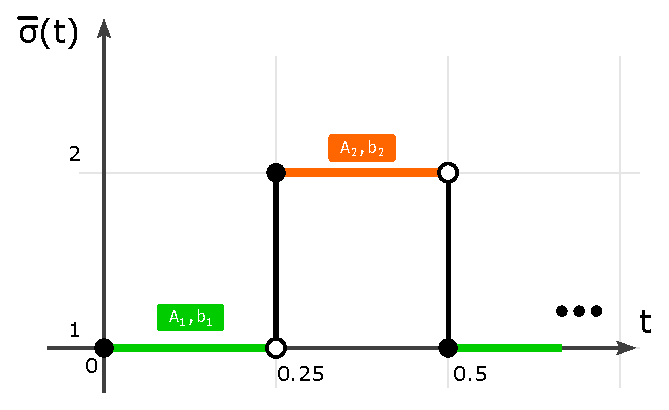
\includegraphics[]{figures/shared/cap4_ref_signal_patino1.eps}
    \caption{Reference sequence for Buck-Boost converter}
    \label{fig:cap4:buck-boost-reference-sequence}
\end{figure}

\noindent
where

\begin{equation}
    \begin{matrix}
        A_1 = \left[ \begin{matrix} 0 & 0 \\ 0 & -1/(RC) \\ \end{matrix} \right], &
        A_2 = \left[ \begin{matrix} 0 & 1/L \\ -1/C & -1/(RC) \\ \end{matrix} \right] \\
        \\
        b_1 = \left[ \begin{matrix} E/L \\ 0 \end{matrix} \right] &
        b_2 = \left[ \begin{matrix} 0 \\ 0 \end{matrix} \right]
    \end{matrix}
    \nonumber
\end{equation}


\noindent
The operation mode is characterized by the index vector \highlight{$\Omega = [1, 2]$}, with 
associated time switch values \highlight{$\tau^\infty = [0, 0.2513, 0.5914] \;\mathrm{s}$}. The 
trajectory is defined by a reference state vector \highlight{$\bar{x}_{ref} = [2 \;\mathrm{V}, -1 
\;\mathrm{A}]$} and a maximum cycle period \highlight{$T_{p_{max}} = 1 \;\mathrm{s}$}. Furthermore, 
the nominal target trajectory originates from the initial state \highlight{$x_0 = [1.8708 
\;\mathrm{V}, -1.1198 \;\mathrm{A}]$}. Simulation parameters include a time step of 
\highlight{$t_{step} = 1 \times 10^{-5} \;\mathrm{s}$} and an identity weight matrix 
\highlight{$Q = I$}.
\subsubsection{Prediction Matrices}

The prediction matrices are constructed using  \eqref{eq:cap4:linearization-phi} and \eqref{eq:cap4:linearization-gamma}, and the result is

\begin{equation}
    \Phi =
    \left[
    \begin{matrix}
        0.9713 & 0.2192 \\
        -0.1707 & 0.5857 
    \end{matrix}
    \right]
\end{equation}

\begin{equation}
    \Gamma =
    \left[
    \begin{matrix}
        2.4556 \\
        0.9280 
    \end{matrix}
    \right]
\end{equation}

with the switching time constraints

\begin{equation}
    c = 
    \left[
        \begin{matrix}
            -\Delta t_{r_1} + \Delta t_{r_{1, min}} \\
            -\Delta t_{r_2} + \Delta t_{r_{2, min}} \\
            \vdots \\
            -\Delta t_{r_{N-1}} + \Delta t_{r_{{N-1}, min}} \\
            -\Delta t_{r_N} + \Delta t_{r_{N, min}} \\
        \end{matrix}
    \right] = 
    \left[
        \begin{matrix}
            - 0.25 + 0.25 \\
            - 0.2504 + 0.25 \\
        \end{matrix}
    \right] =
    \left[
        \begin{matrix}
            0 \\
            - 0.04 \\
        \end{matrix}
    \right]
\end{equation}

\subsubsection{Results}

Figure \ref{fig:cap4:buck-boost-feasibility-region} presents the feasibility region \highlight{$\mathcal{D}$} for three different prediction horizons 
($N_p = 1$, $N_p = 2$ and $N_p = 3$) for the Buck-Boost Converter.

\begin{figure}[!ht]
    \centering
    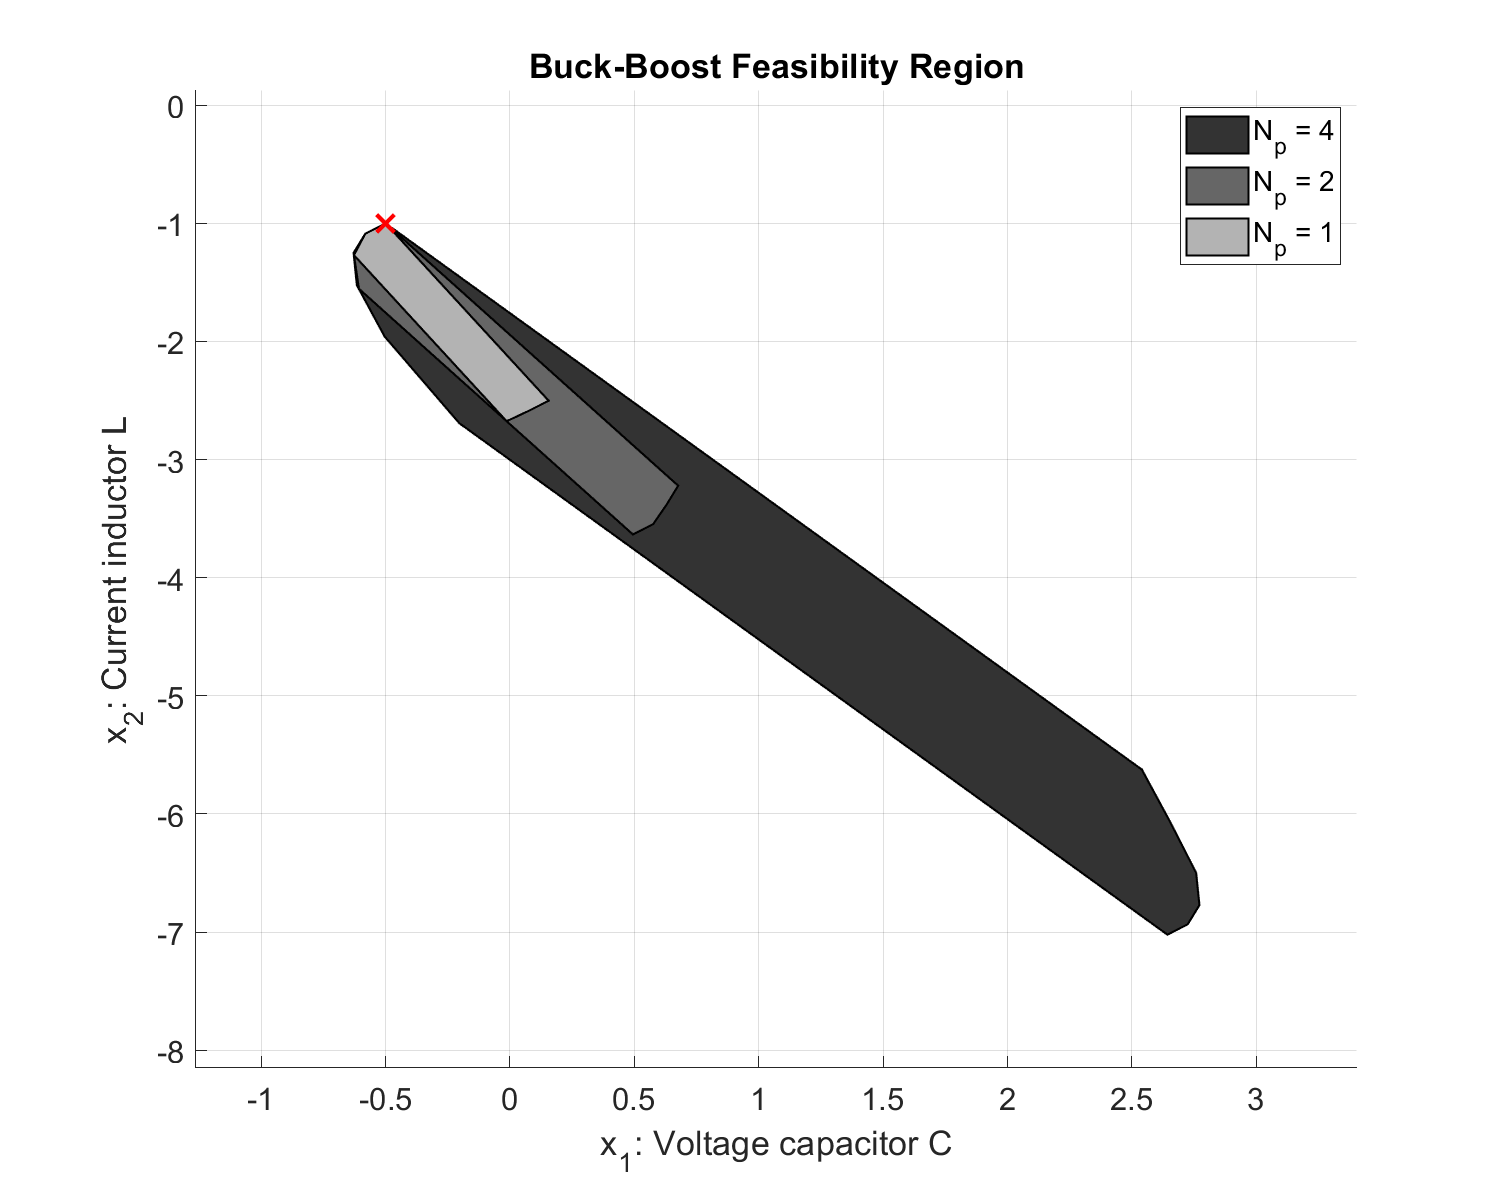
\includegraphics[width=14cm]{figures/cap4/graf_proj_patino1.pdf}
    \caption{Buck-Boost Feasibility Region}
    \label{fig:cap4:buck-boost-feasibility-region}
\end{figure}


Figure \ref{fig:cap4:buck-boost-state-trajectory} shows the simulation of the trajectory for the system
, \highlightblue{in blue} we see the trajectory without using the MPC controller, and 
\highlightorange{in orange} we see the trajectory using the MPC controller.
They are both starting from \highlight{$x_0 = \big[2.0493 \;\mathrm{V},-0.6108 \;\mathrm{A}\big]$} 
and converge to the initial position of the target cyclic trajectory 
\highlight{$\bar{x}_0 = \big[1.8493 \;\mathrm{V}, -1.1108 \;\mathrm{A}\big]$}. Note that 
the trajectory with the MPC controller converges faster to the 
cyclic trajectory.

Figure \ref{fig:cap4:buck-boost-control-signal} shows the control signal sequence, where we can see that the difference between the nominal 
target trajectory and the controlled trajectory decrease as they get in sync with each other. 

\begin{figure}[H]
    \centering
    
\includegraphics[width=12cm]{figures/cap4/graf_patino1_traj.pdf}
    \caption{State Trajectory for Buck-Boost converter}
    \label{fig:cap4:buck-boost-state-trajectory}
\end{figure}

\begin{figure}[H]
    \centering
    
\includegraphics[width=12cm]{figures/cap4/graf_patino1_u_signal.pdf}
    \caption{Control Signal Sequence for Buck-Boost converter}
    \label{fig:cap4:buck-boost-control-signal}
\end{figure}
